\documentclass[11pt,a4paper]{article}
\usepackage{fontspec}
\setmainfont{Source Serif 4}[Path=/home/claude/ref/fonts/, UprightFont=SourceSerif4-Regular.ttf, BoldFont=SourceSerif4-Semibold.ttf, ItalicFont=SourceSerif4-It.ttf]
\setmonofont{IBM Plex Mono}[Path=/home/claude/ref/fonts/, UprightFont=IBMPlexMono-Regular.ttf, BoldFont=IBMPlexMono-Medium.ttf, Scale=0.88]
\usepackage[a4paper,margin=2.4cm]{geometry}
\usepackage{amsmath}
\usepackage{graphicx,booktabs,float,caption,array,xcolor,longtable}
\usepackage{xurl}
\usepackage[hidelinks]{hyperref}
\usepackage[round]{natbib}
\usepackage{setspace}
\setstretch{1.08}
\renewcommand{\topfraction}{0.9}
\renewcommand{\bottomfraction}{0.8}
\renewcommand{\textfraction}{0.1}
\renewcommand{\floatpagefraction}{0.75}
\setlength{\parindent}{0pt}
\setlength{\parskip}{0.55em}
\captionsetup{font=small,labelfont=bf}
\setlength{\bibsep}{3pt}
\urlstyle{same}
\hypersetup{pdftitle={Can You See the Sea?},pdfauthor={Dr Tristan Hotham}}

\begin{document}
\begin{center}
{\Large\bfseries Can You See the Sea? A Line-of-Sight Census of Sea Views from Every 1 km Square of the United Kingdom\par}
\vspace{1.2em}
{\large Dr Tristan Hotham\par}
\vspace{0.3em}
{\small Independent researcher\\
ORCID: 0000-0003-4931-9349\\
DOI: https://doi.org/10.5281/zenodo.24106076\par}
\vspace{0.8em}
2026
\end{center}

\begin{quote}
\small
\begin{center}\textbf{Abstract}\end{center}
Sea views are prized in housing markets and linked to well-being, yet I have found no estimate of how much of any country can see the sea. I compute a line-of-sight census for every 1~km square of the United Kingdom (244,595 squares): 360 sight lines from each square centre over the open AWS Terrain Tiles (about 175~m) to 50~km, with Earth curvature and standard refraction, against an OpenStreetMap sea mask in which ``sea'' includes tidal estuaries and sea lochs. Standing on bare ground with eyes 1.7~m up, the sea is in view from 26.3\% of UK land: 41.3\% of Scotland, 33.6\% of Wales, 22.5\% of Northern Ireland and 16.4\% of England, rising to 29.2\% at 5~m and 45.1\% at 50~m. Half of low-lying squares lose sight of the sea within 3.5~km of the coast (95\% CI 3.1 to 3.9), against 9.0~km on ground of 150 to 300~m. About 23\% of Great Britain's population lives at settlement points with a sea view. The square farthest from any sea view is 94~km from one, in Leicestershire. Every analysis and check was pre-specified in a written plan. The model reproduces 9 of 10 documented summit sea views. All figures are upper bounds, for bare terrain without buildings or trees. The headline is also resolution-sensitive: finer terrain (about 88~m) lowers the share in all four test windows, by up to 7.3 points.

\textbf{Keywords:} viewshed; line of sight; sea view; coast; visibility; terrain analysis; United Kingdom
\end{quote}

\section{Introduction}
``Sea views'' is a phrase estate agents use to sell homes. Hedonic studies find that a view of water adds to the price of a home \citep{benson1998,bourassa2004,jim2009}, and a growing literature in environmental psychology and public health associates the sight of water, and living near the coast, with better mood and health \citep{white2010,wheeler2012,nutsford2016,gascon2017}. Yet I have not found an answer, for any whole country, to the basic geographical question behind all of this: from how much of the land can you actually see the sea?

The question sounds simple and is not. Whether the sea is visible from a point depends on the terrain between the observer and the coast, on the observer's height, on the curvature of the Earth, which hides a distant sea surface below the horizon, and on atmospheric refraction, which bends sight lines and lifts it back a little. It depends on what counts as ``sea'' (an estuary? a sea loch?) and on how far one is prepared to look. And it depends on everything that stands on the ground: buildings, trees and hedges, which national terrain models largely do not contain. Viewshed analysis, the computation of what is visible from a point over a digital elevation model (DEM), is the standard tool \citep{defloriani2003}, and its sensitivity to these choices has been studied since the work of \citet{fisher1991,fisher1992,fisher1993}.

This paper computes a line-of-sight census of sea views for the whole United Kingdom: every Ordnance Survey National Grid 1~km square of Great Britain and every Irish Grid 1~km square of Northern Ireland, 244,595 in all. From the centre of each square I trace 360 sight lines, one per degree of azimuth, across open terrain data to 50~km, allowing for curvature and standard refraction, and record whether any part of the sea surface is in view, how far away the nearest visible sea is, and what share of the horizon is sea. The same computation at four eye heights (standing, an upstairs window, a fifth floor and a tall tower) shows how much height buys. Settlement points from Wikidata, weighted by census populations, give the share of people living where the sea is in view. Named viewpoints with documented sea views provide an external check.

The contribution is threefold. First, it provides a complete national estimate, of a kind I have not found published elsewhere, of the land area and population with a terrain sea view in the United Kingdom, at a resolution that resolves individual coastal hills and valleys. Second, it gives a simple, reusable measure for research on coastal amenity and blue space: a per-square indicator, a distance to the nearest visible sea and a share of the horizon, released as open data. Third, it quantifies how sensitive such a measure is to the choices that viewshed research has long warned about: observer height, maximum distance, refraction, the definition of the sea, the resolution of the terrain and its errors. Every analytic choice and check was pre-specified in a written plan before any visibility result was computed (Section~\ref{sec:design}); the plan is released with the code.

The rest of the paper is organised as follows. Section~\ref{sec:lit} reviews viewshed analysis and the literature on coastal views. Section~\ref{sec:data} describes the data, Section~\ref{sec:design} the method and the plan. Section~\ref{sec:results} reports the results and Section~\ref{sec:robust} the validation and robustness checks. Section~\ref{sec:disc} discusses limitations and uses, and Section~\ref{sec:conc} concludes.

\section{Background and literature}\label{sec:lit}
\subsection{Viewsheds and their uncertainty}
A viewshed is the set of locations visible from an observer over a terrain model, or, in its reverse form, the set of observers that can see a target. Algorithms range from tracing an independent sight line to every cell, through sweeps that reuse partial results, to approximations that propagate a reference plane outwards \citep{franklin1994,vankreveld1996,wang1996,wang2000,defloriani2003}. \citet{wang1996} rule out many target cells without tracing a sight line to each, and \citet{wang2000} generate viewsheds ``without using sightlines'' at all; exact sight-line tracing is slower but transparent. With large grids, efficient implementations matter \citep{tabik2013}. The problem solved here is narrower than a full viewshed: for each observer I only need to know whether, and where, a sight line first reaches visible sea. That makes it possible to trace exact sight lines and to stop each one early (Section~\ref{sec:design}).

Viewsheds are notoriously sensitive. \citet{fisher1991} added simulated error fields to a DEM and found that the viewshed area computed on the original DEM may significantly overestimate the viewshed area; \citet{fisher1992} cumulated the Boolean viewsheds from many such error realisations into a fuzzy viewshed. \citet{fisher1993} showed that design choices in viewshed algorithms, above all how the viewpoint and the target are represented, change the viewable area, and that different GIS implementations of the ``same'' operation disagree. \citet{fisher1994} distinguished probable from fuzzy models of the viewshed, and \citet{fisher1996} discussed extending viewsheds for landscape planning. In built-up areas, how buildings' locations and heights are represented changes computed viewsheds significantly \citep{sander2007}. These lessons shape the checks used here: two DEM resolutions, Monte Carlo DEM error in the manner of \citet{fisher1991,fisher1992}, several maximum distances and refraction coefficients, and a frank statement that the result is a bare-terrain upper bound.

Visibility has also been used as a variable in landscape and archaeological research: cumulative viewsheds count how many sites see a cell \citep{wheatley1995}, and planning studies use visibility to assess visual impact \citep{bishop2003}. Isovist analysis applies the same idea in built space \citep{benedikt1979}. The present study is closest to the cumulative viewshed in spirit, but its target is a single, very large feature: the sea.

\subsection{Curvature, refraction and the sea horizon}
Over distances of tens of kilometres the Earth's curvature matters. A target at distance $d$ appears lower than it would on a flat Earth by $d^2/(2R)$, where $R$ is the Earth's radius; atmospheric refraction near the ground usually bends sight lines downwards and reduces this drop. The usual correction replaces $R$ by an effective radius $R' = R/(1-k)$ with a refraction coefficient $k$ of about 0.13, the standard value in geodetic levelling, although measurements about 1.8~m above the ground show $k$ varying strongly with the temperature gradient and over the day, so that the constant 0.13 describes near-ground refraction poorly \citep{hirt2010}. For the sea, curvature has a second role: a calm sea surface is itself the horizon. From an eye at height $H$ above the sea, the sea surface at distance $d$ is seen at an angle $-H/d - d/(2R')$ below the horizontal, which is highest at the sea-horizon distance $d^\ast = \sqrt{2HR'}$ (about 5~km for an eye 1.7~m above sea level and 140~km for one 1,300~m up) and falls beyond it. A sea surface beyond $d^\ast$ is never visible however clear the air, and any land that rises above the angle of the sea horizon, $-\sqrt{2H/R'}$, hides all the sea behind it. Both facts are used to stop sight lines early.

\subsection{Why sea views matter}
Three literatures motivate a national measure. In housing economics, hedonic studies estimate the premium for views: \citet{benson1998} price ocean and lake views in Bellingham, Washington, \citet{bourassa2004} ask ``what's in a view?'' in Auckland and find that the value of a water view depends on its scope and distance, and \citet{jim2009} value scenic views in Hong Kong. In England, \citet{gibbons2014} estimate the amenity value of habitats, designated areas, water and other natural features for house prices, using distances and shares of land rather than lines of sight. In health research, ``blue space'' studies associate coastal proximity and visible water with better health and well-being: \citet{white2010} found that scenes with water were preferred and rated more restorative, \citet{wheeler2012} that good health is more prevalent near the coast in England, \citet{nutsford2016} that visible blue space, measured with geospatial visibility techniques, was associated with lower psychological distress in Wellington, and \citet{garrett2019} that the association between coastal proximity and mental health in urban England is moderated by income; reviews by \citet{volker2011} and \citet{gascon2017} summarise the evidence. Many of these studies use distance to the coast, a proxy that ignores whether the sea is actually in view. Third, in landscape research viewshed mapping is central to assessing views and visual impact \citep{bishop2003}.

\subsection{What is new here}
Previous work has computed visible water for a single city \citep{nutsford2016} or for samples of homes in hedonic models, and earlier studies by the author computed horizons for UK settlements \citep{hotham2026sunless} and sea sunsets from beaches \citep{hotham2026sunsets}. I am not aware of a published national estimate of the land area or population with a sea view for the United Kingdom or any comparable country. This paper provides one, with a transparent method, open data and code, an analysis pre-specified in a written plan, and checks against both documented views and alternative modelling choices.

\section{Data}\label{sec:data}
\subsection{Terrain}
Terrain heights come from the AWS Terrain Tiles \citep{terraintiles}, a global mosaic in the ``Terrarium'' PNG encoding assembled by Mapzen from SRTM \citep{farr2007}, GMTED2010 \citep{gmted}, ETOPO1 \citep{etopo1} and other sources \citep{joerd}. I use zoom level 9, tiles $x$ 244 to 258 and $y$ 145 to 174 (450 tiles), which cover Britain, Ireland and the near Continent at a pixel size of about 196~m at 50\textdegree{}N and 150~m at 61\textdegree{}N in Web Mercator. Following the sister study of winter sunshine \citep{hotham2026sunless}, isolated spikes and pits were replaced by the median of their $7\times7$ neighbourhood (143 cells). The terrain is a surface model in the sense of the SRTM radar, which partly sees woodland and buildings, smoothed to the tile resolution: summits are lower than their surveyed heights and narrow ridges are softened. SRTM's absolute vertical error was assessed globally by \citet{rodriguez2006}.

\subsection{The sea}
The sea is OpenStreetMap's coastline \citep{osm,haklay2010}, taken from the water layer (class ``ocean'') of the OpenFreeMap vector tiles \citep{openfreemap} at zoom 9 (release 20261101\_080013\_pt) and rasterised onto the terrain pixels. OpenStreetMap's coastline follows mean high water and runs up tidal estuaries, so the Thames, Humber and Severn estuaries and the sea lochs of western Scotland count as sea; a planned check removes channels narrower than about a kilometre (Section~\ref{sec:design}). Sea pixels are given a height of 0~m; land pixels keep the terrain height, including the Fens and other land a little below sea level.

\subsection{Squares, settlements and population}
The observers are the centres of the Ordnance Survey National Grid 1~km squares of England, Scotland and Wales and the Irish Grid 1~km squares of Northern Ireland whose centre is not sea and lies within, or within 2~km of the coast of, a UK nation polygon (ONS-derived counties). This gives 230,336 squares in Great Britain and 14,259 in Northern Ireland, close to the published areas of the two (a square stands for 1~km$^2$; inland water is included). Each square also carries its distance to the coast (to the nearest sea pixel), its terrain height and its local relief (height minus the mean land height within about 5~km).

Settlements come from Wikidata \citep{wikidata}: the 36,692 living UK settlements with coordinates assembled for \citet{hotham2026sunless}, 13,767 of them with a population. Wikidata populations overlap (a city and its suburbs are listed separately) and are of mixed dates, so they are used only to weight settlements within a parliamentary constituency. Constituency populations are those of the 2011 Census for the 632 Westminster constituencies of Great Britain as drawn in 2010, with their boundaries, as compiled for earlier studies by the author.

\subsection{Viewpoints with documented sea views}
For validation I collected named summits and viewpoints whose sea view is stated in a published or online source: Black Combe, Dunkery Beacon, Pendle Hill, Leith Hill (from its tower), Ditchling Beacon, Brown Willy, Worcestershire Beacon, Snowdon, Scafell Pike and Slieve Donard (Table~\ref{tab:valid}). Where the source says only that a distant coast or island is visible across the sea (Snowdon, Scafell Pike, Slieve Donard), I take the sea between as visible. The quotations and sources are in the released data. Positions are the published grid references.

\section{Method and analysis plan}\label{sec:design}
\subsection{Sight lines}
For an observer at a square centre with terrain height $g$ and eye height $e$, so that $H=g+e$, I trace 360 rays at azimuths $0^\circ, 1^\circ, \dots, 359^\circ$. Rays are marched in the Web Mercator pixel grid of the terrain in steps of half a pixel (about 90~m), with the true ground distance accumulated from the local pixel size at each step, so the scale change with latitude is handled exactly. At each step the terrain height $h$ is interpolated bilinearly, or set to 0 if the nearest pixel is sea, and its apparent elevation is
\[ a(d) = \frac{h-H}{d} - \frac{d}{2R'}, \qquad R' = \frac{R}{1-k}, \]
with $R = 6{,}371$~km and $k = 0.13$. A sea sample is visible if its $a$ is at least the largest $a$ of every sample nearer along the ray; the ray then stops and records the distance. It also stops at 50~km, at the edge of the terrain mosaic (493 rays out of more than 87 million, all from western Northern Ireland towards Donegal; they are counted as seeing no sea), or as soon as the running maximum exceeds the highest angle that any farther sea surface could reach: $-\sqrt{2H/R'}$ before the sea-horizon distance and the sea's own angle beyond it. This stopping rule is exact, not an approximation: no sea beyond such a point can be visible. Because a sea sample on the ray must also clear the nearer sea surface, the curvature of the sea itself is handled automatically. The kernel is compiled with Numba and runs in a few minutes for the whole country on two processor cores.

\subsection{Outcomes and estimands}
For each square the outcomes are: whether the sea is visible on any ray (``sea view''); the distance to the nearest visible sea (the minimum over rays); and the share of the 360 rays that reach visible sea (``share of the horizon''). The planned estimands were: E1, the share of UK land squares with a sea view at 1.7~m, by nation; E2, the share of population with a sea view; E3, the distance inland at which half of squares see the sea, by terrain height band (0 to 50, 50 to 150, 150 to 300 and over 300~m), estimated from the share of squares with a sea view in 1~km bands of distance to the coast (smoothed over three bands) and given 95\% intervals by a block bootstrap over 50~km grid blocks (1,000 replicates); E4, the squares farthest from any square with a sea view and the square farthest from the coast; and E5, the distribution of distances and horizon shares.

For E2, each Great Britain constituency's 2011 population is split by the share of its Wikidata settlement population whose own settlement point has a sea view. Settlements whose Wikidata population exceeds their constituency's census population are aggregates (urban areas, counties) and are dropped (93 entries); constituencies with no settlement population (7) fall back to their share of squares with a sea view. Northern Ireland, which lacks the constituency data here, is weighted by Wikidata settlement population directly. Each settlement point is computed exactly, not taken from its square.

\subsection{A descriptive model}
To summarise what goes with a sea view, the plan specified a logistic regression (M1) of the square's sea view on a natural cubic spline in the log of distance to the coast (four degrees of freedom), $\log(1+\text{height})$, local relief, and nation fixed effects, with standard errors clustered by 50~km grid block. It is descriptive: it shows how the probability of a sea view varies with geography, not why. Effects are reported as average marginal effects (percentage points) with 95\% intervals from 300 draws from the clustered covariance matrix.

\subsection{Planned checks}
The plan fixed the following checks and decision rules before the results were seen. V1, validation: the model must reproduce at least 80\% of the documented sea views at the terrain's own height, or every result is labelled provisional; it is also run at the published summit height (the zoom-9 terrain flattens summits). S1, eye heights of 5, 15 and 50~m. S2, maximum distances of 25 and 100~km. S3, refraction coefficients of 0 and 0.25. S4, 720 rays (every half degree) for a random 5\% of squares. S5, a 500~m grid: four quarter-points per square for a random quarter of squares (reduced from all squares, as planned, to keep the computation bounded on a shared machine). S6, terrain resolution: zoom-10 tiles (about 88~m) in four test windows (squares within 50~km of a centre on the Cumbria and Lancashire coast, in Cornwall, in Lothian and Fife, and in Norfolk), with the rule that a difference of more than 3 percentage points in any window makes the headline resolution-sensitive. S7, open sea only: ocean pixels in channels narrower than about 1.2~km (a morphological opening) do not count as sea. S8, more than a glimpse: the sea must be visible on at least 3 of the 360 rays. S9, terrain error in the manner of \citet{fisher1991,fisher1992}: for 2,000 random squares, 20 realisations of spatially correlated Gaussian error (standard deviation 5~m and, as a variant, 10~m; correlation length about 1~km) added to the land. The plan also stated what would count against the method: failed validation, large resolution sensitivity, or a farthest-from-the-sea point far from the published one.

\section{Results}\label{sec:results}
\subsection{How much of the UK sees the sea}
Standing on the bare ground, with eyes 1.7~m up, the sea is in view within 50~km from 64,277 of the UK's 244,595 squares: 26.3\% of the land (Figure~\ref{fig:map}, Table~\ref{tab:nations}). The shares differ greatly by nation. Scotland, with its long, indented and mountainous coast, sees the sea from 41.3\% of its land, Wales from 33.6\%, Northern Ireland from 22.5\% and England from only 16.4\%. England's broad lowland interior, much of it more than 50~km from any coast, accounts for most of the UK's land without a sea view.

\begin{figure}[tbp]\centering
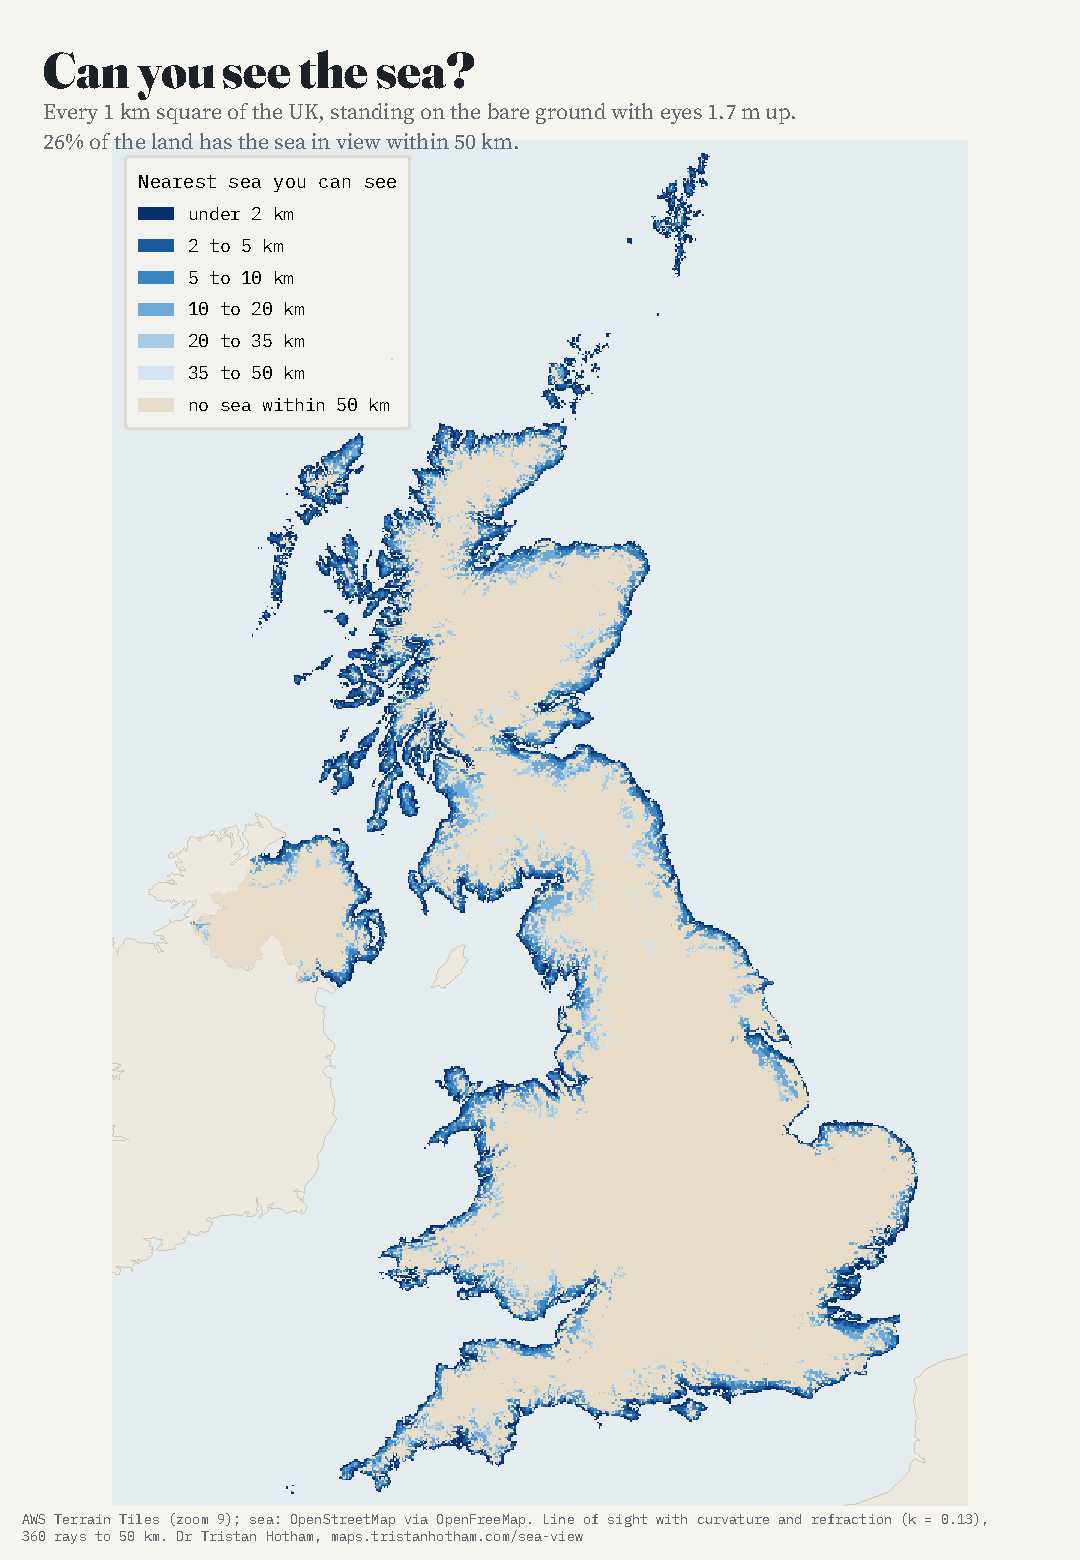
\includegraphics[width=0.78\textwidth]{f_map.pdf}
\caption{Distance to the nearest visible sea from every 1~km square of the United Kingdom, eyes 1.7~m above bare terrain, sight lines to 50~km. Sand: no sea in view. Ireland, the Isle of Man and France are shown for context and were not computed.}\label{fig:map}
\end{figure}

\begin{table}[tbp]\centering\small\caption{Land with a sea view by nation and eye height: squares (km$^2$), squares with a sea view at 1.7~m, and the share (\%) at each eye height. Sight lines to 50~km, $k=0.13$.}\label{tab:nations}\begin{tabular}{lrrrrrr}\toprule & Squares & Sea view & \multicolumn{4}{c}{Share with a sea view (\%), eyes at}\\\cmidrule(lr){4-7} Nation & (km$^2$) & at 1.7~m & 1.7~m & 5~m & 15~m & 50~m\\\midrule
England & 130,646 & 21,470 & 16.4 & 19.5 & 25.1 & 36.2\\
Scotland & 78,911 & 32,615 & 41.3 & 44.3 & 49.4 & 59.2\\
Wales & 20,779 & 6,985 & 33.6 & 36.6 & 41.9 & 53.2\\
Northern Ireland & 14,259 & 3,207 & 22.5 & 24.7 & 28.7 & 37.0\\
\midrule United Kingdom & 244,595 & 64,277 & 26.3 & 29.2 & 34.5 & 45.1\\
\bottomrule\end{tabular}\end{table}

Where the sea is in view it is usually close. The median distance to the nearest visible sea, among squares that have one, is 5.9~km (interquartile range 2.0 to 14.8~km). Most views are partial: among squares with a sea view, a median of 14.2\% of the 360 sight lines reach visible sea, and 41\% see the sea across less than a tenth of the horizon. Only 2,789 squares (1.1\% of the land) look out on sea across more than half the horizon: headlands, small islands and the narrow ends of peninsulas (Figure~\ref{fig:horizon}).

\begin{figure}[tbp]\centering
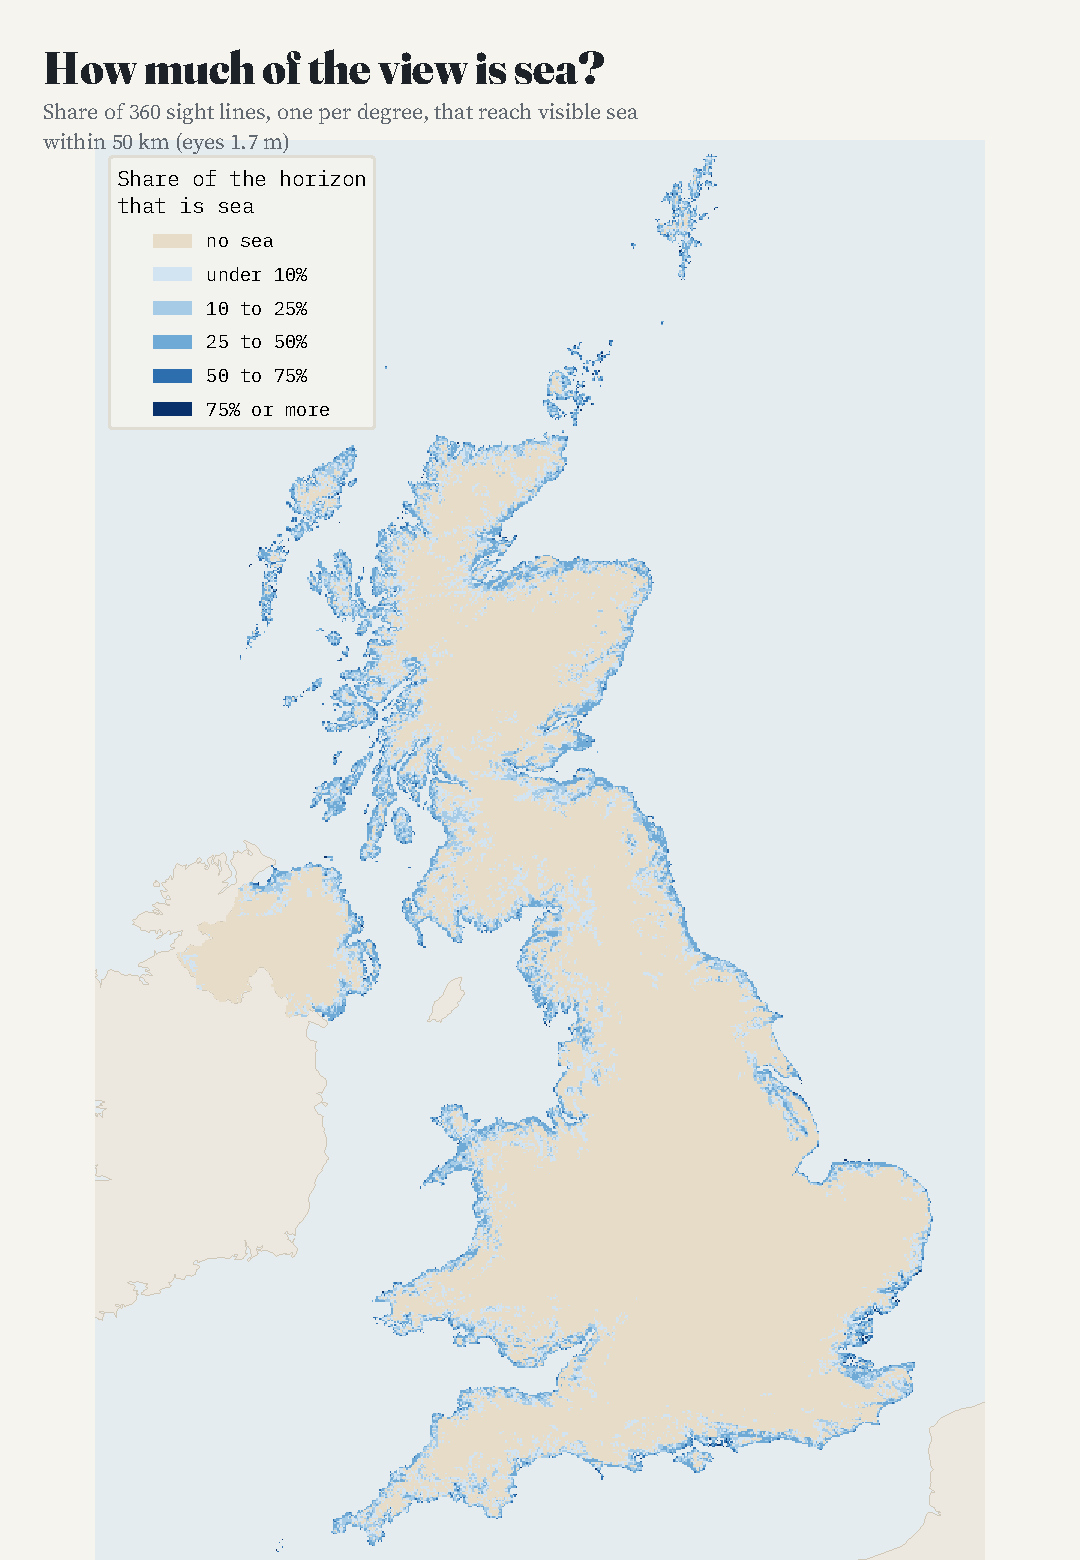
\includegraphics[width=0.66\textwidth]{f_horizon.pdf}
\caption{Share of the horizon that is sea: the share of 360 sight lines that reach visible sea within 50~km, eyes 1.7~m.}\label{fig:horizon}
\end{figure}

Height buys sea. At an upstairs window (5~m above the ground) the share of UK land with a sea view rises to 29.2\%, at a fifth floor (15~m) to 34.5\% and at the top of a 50~m tower to 45.1\% (Figure~\ref{fig:eyes}). The heights are applied everywhere, including open moorland, so they show the potential of a tall building rather than any actual one.

\begin{figure}[tbp]\centering
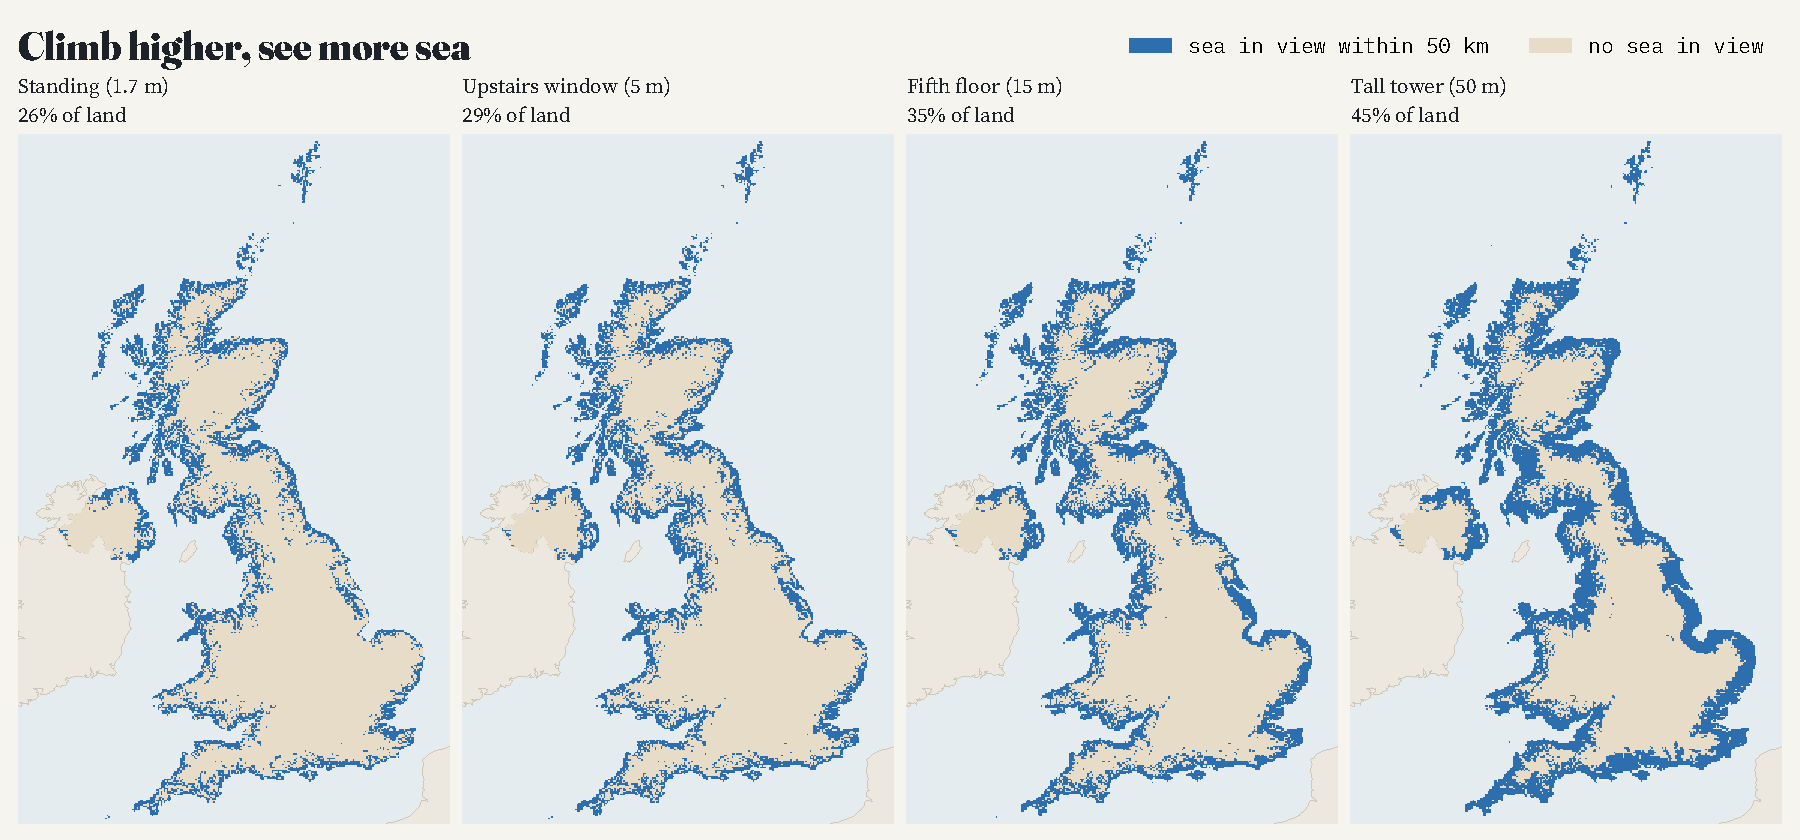
\includegraphics[width=\textwidth]{f_eyes.pdf}
\caption{Squares with the sea in view within 50~km for four eye heights above the bare terrain.}\label{fig:eyes}
\end{figure}

\subsection{How far inland the sea stays in view}
Distance from the coast is the strongest correlate, but it is not the whole story (Figure~\ref{fig:profile}). Of squares within a kilometre of the coast, 97.6\% see the sea; at 2 to 5~km, 68.4\%; at 10 to 20~km, 22.0\%; and at 30 to 50~km, 1.9\%. Conversely, 7.1\% of squares within 2~km of the coast have no sea view at all, hidden behind dunes, cliffs, sea walls or the slope of the land.

Height above sea level sets how far the view reaches inland (Table~\ref{tab:reach}). On land below 50~m, half of squares have lost sight of the sea by 3.5~km from the coast (95\% CI 3.1 to 3.9); on land between 50 and 150~m by 6.5~km (5.8 to 7.3); between 150 and 300~m by 9.0~km (8.1 to 10.2); and above 300~m by 8.6~km (7.1 to 13.6). The highest band gains nothing over the one below it at the half-way mark, because most land above 300~m lies in the Highlands, the Southern Uplands, the Lake District and Snowdonia, where neighbouring mountains block the view; but beyond about 10~km it keeps a sea view more often than any other band, and 80 squares above 300~m see the sea from 40~km or more inland (Figure~\ref{fig:profile}).

\begin{figure}[tbp]\centering
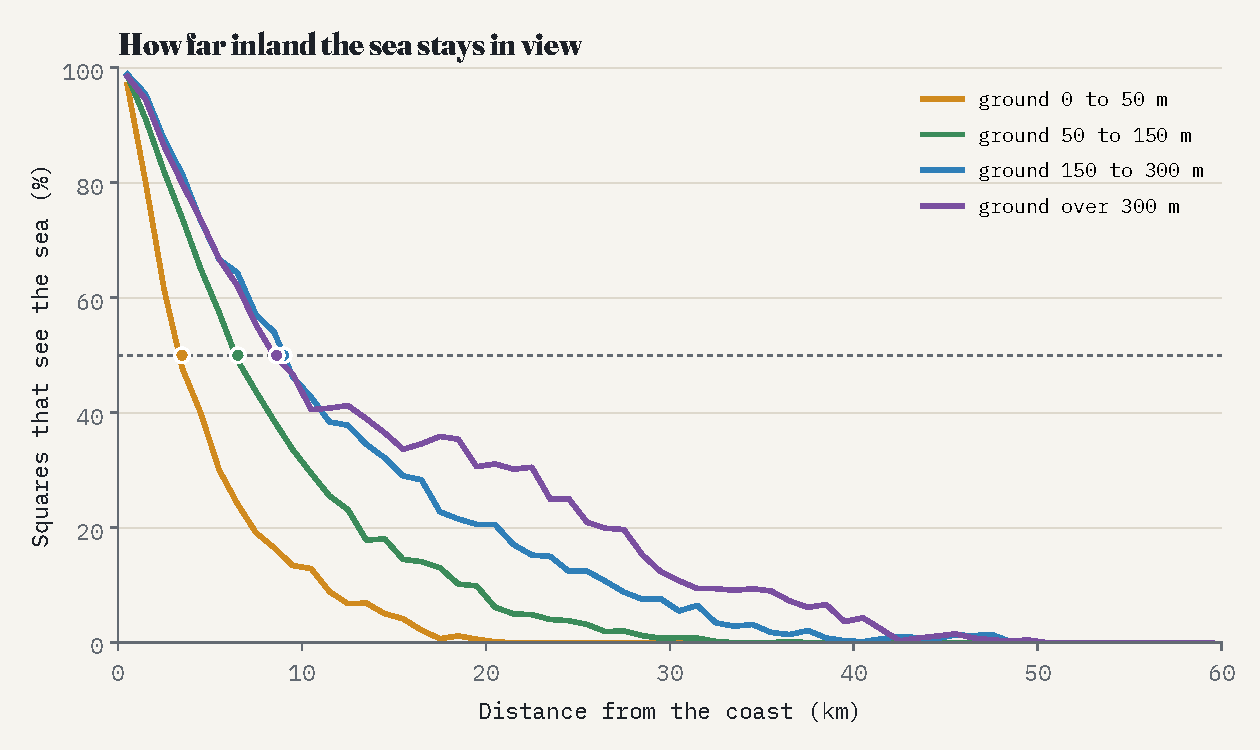
\includegraphics[width=0.85\textwidth]{f_profile.pdf}
\caption{Share of squares with a sea view by distance from the coast (1~km bands, at least 30 squares) and terrain height band. Dots: the distance at which the smoothed share falls below a half (Table~\ref{tab:reach}).}\label{fig:profile}
\end{figure}

\begin{table}[tbp]\centering\small\caption{How far inland the sea stays in view: the distance from the coast at which the share of squares with a sea view (1~km bands, smoothed over three bands) falls below a half, by terrain height. 95\% intervals from a block bootstrap over 50~km grid blocks (1,000 replicates).}\label{tab:reach}\begin{tabular}{lrrrl}\toprule Terrain height & Squares & Sea view (\%) & Half-way distance (km) & 95\% CI\\\midrule
0 to 50 m & 59,203 & 32.9 & 3.5 & [3.1, 3.9]\\
50 to 150 m & 92,151 & 23.3 & 6.5 & [5.8, 7.3]\\
150 to 300 m & 53,942 & 26.4 & 9.0 & [8.1, 10.2]\\
Over 300 m & 39,299 & 23.1 & 8.6 & [7.1, 13.6]\\
\midrule All squares & 244,595 & 26.3 & 6.0 & [5.4, 6.6]\\
\bottomrule\end{tabular}\end{table}

The descriptive model M1 confirms the pattern (244,595 squares, 176 clusters; Appendix Table~\ref{tab:m1}). Holding distance to the coast and nation as observed, raising every square by 100~m of terrain height changes the share with a sea view by 4.7 percentage points (95\% CI 3.8 to 5.7), and standing 50~m higher than the surrounding land (local relief) by 3.7 points (2.7 to 4.5). Setting every square at 5~km from the coast, the model predicts a sea view from 57.3\% of squares (53.5 to 60.9); at 20~km, 13.4\% (11.0 to 15.9).

\subsection{People}
Most people in Great Britain live in lowland towns and cities, many of them inland, and those on the coast often look across flat land or estuaries. Splitting each constituency's 2011 population by the share of its settlement population whose point sees the sea, 22.6\% of people in Great Britain (about 13.9 million of 61.4 million) live at settlement points with a sea view from 1.7~m; with eyes at an upstairs window, 25.2\%; at 15~m, 29.9\%; at 50~m, 37.7\% (Figure~\ref{fig:nations}). Weighting by Wikidata populations alone, without the census, gives 22.0\%; counting settlements without weights, 26.7\% of the 36,692 settlement points see the sea. In Northern Ireland, 56.0\% of the Wikidata settlement population does. Of the 634 places with at least 20,000 people in Wikidata (aggregates excluded), 21.9\% see the sea from their point. These figures describe a point per settlement on bare terrain; they say nothing about which homes have a view.

\begin{figure}[tbp]\centering
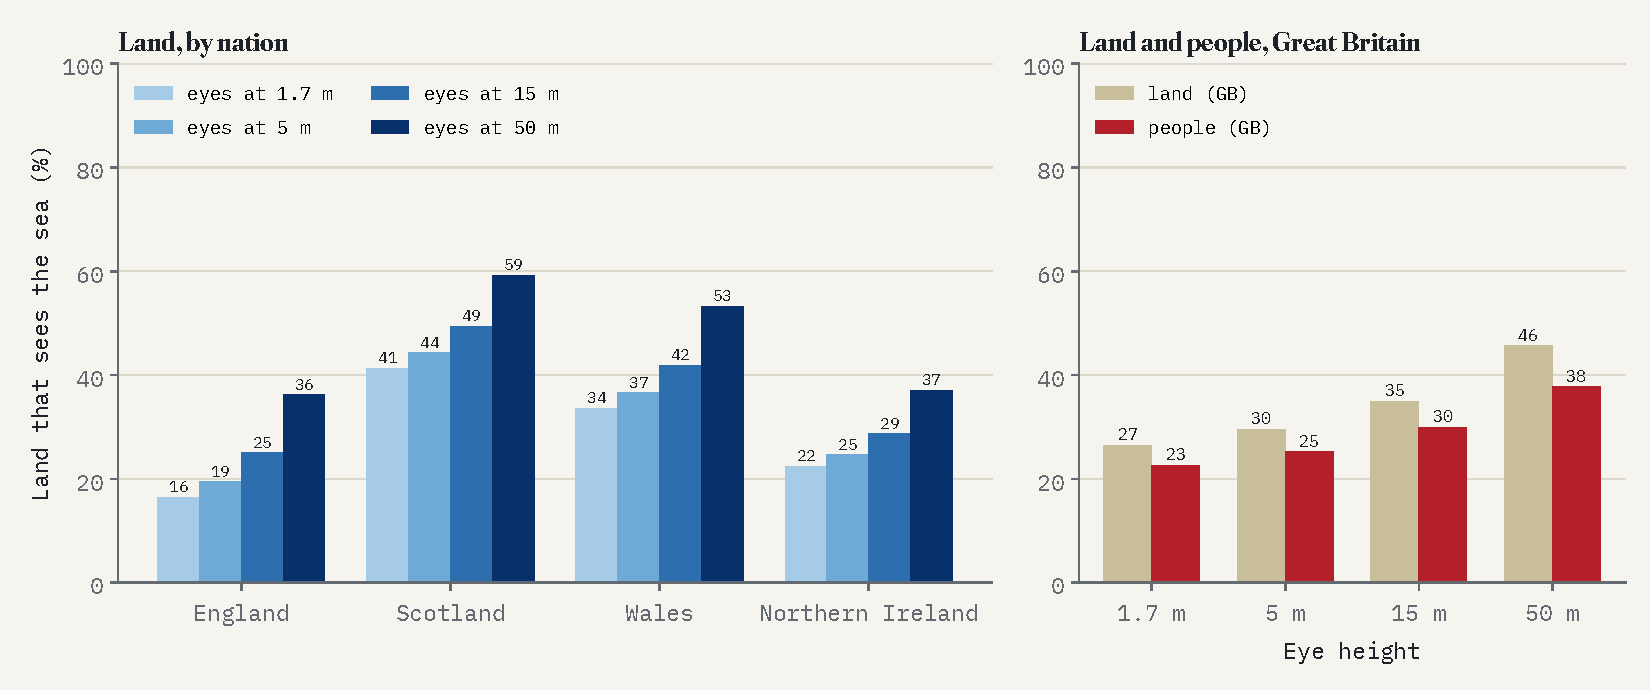
\includegraphics[width=\textwidth]{f_nations.pdf}
\caption{Left: share of land with a sea view by nation and eye height. Right: share of land and of people in Great Britain with a sea view, by eye height (people: 2011 Census by 2010 constituency, split by settlement points).}\label{fig:nations}
\end{figure}

\subsection{Far from any sea view}
The land square farthest from any square with a sea view lies 94.4~km from one, near Donington le Heath in Leicestershire (Figure~\ref{fig:farthest}). The square farthest from the coast itself is 114.4~km from the nearest sea pixel, near Akeley (Buckinghamshire). Both lie in lowland inland England, where a wide area has no sea view from any square within tens of kilometres; 18 of the 88 counties and council areas have no square with a sea view at all (Appendix Table~\ref{tab:counties}). At the other extreme, the square with a sea view farthest from the coast is 49.7~km inland, near Hope (Durham), at 426~m: right at the 50~km limit of the sight lines.

\begin{figure}[tbp]\centering
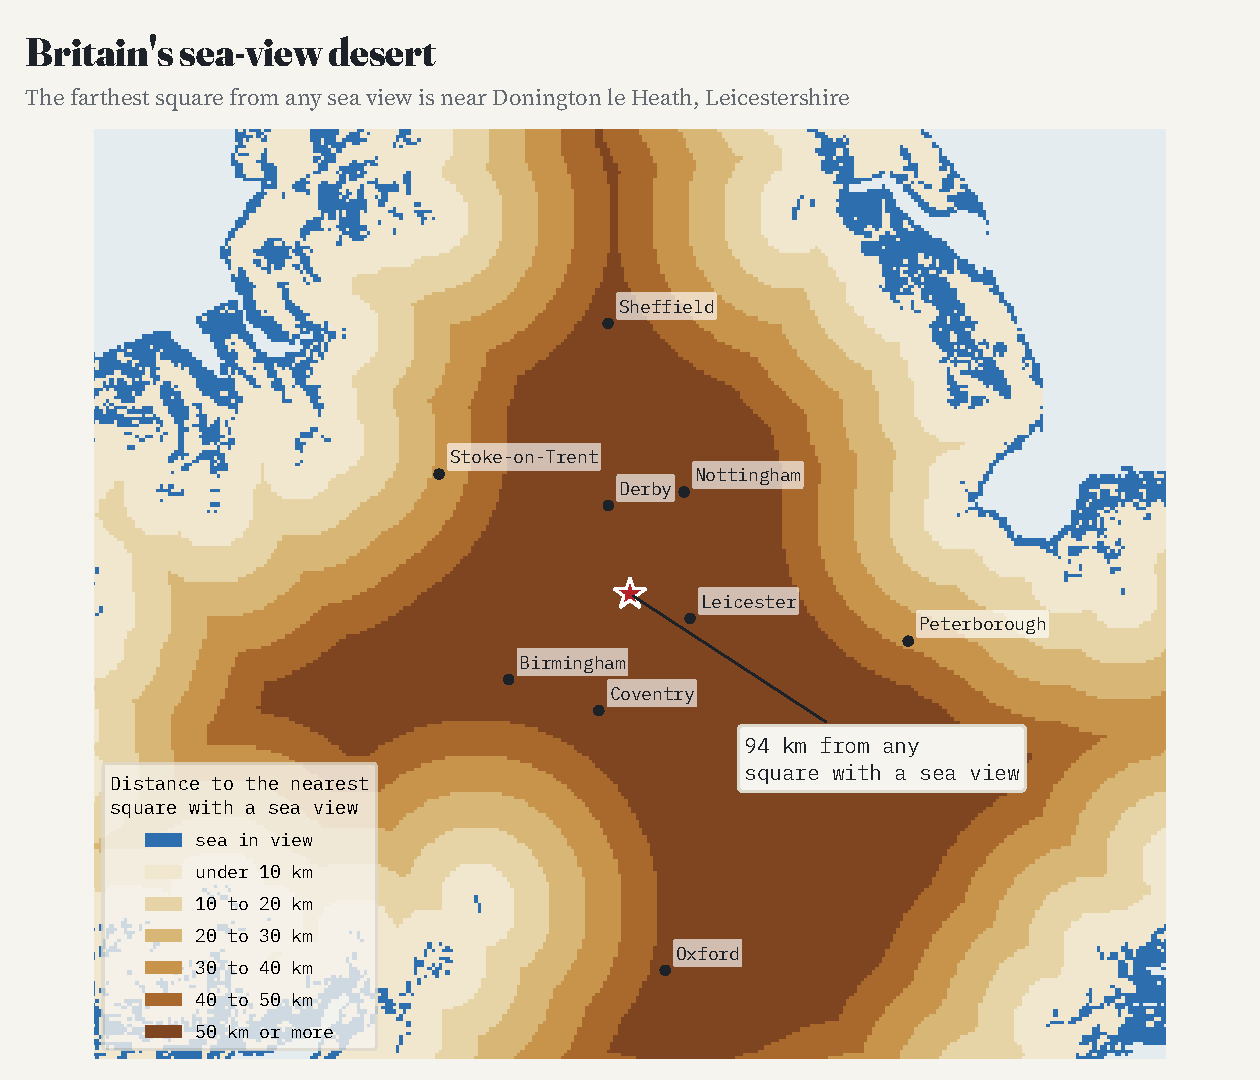
\includegraphics[width=0.85\textwidth]{f_farthest.pdf}
\caption{Distance from each square to the nearest square with a sea view, central England, with the farthest square marked.}\label{fig:farthest}
\end{figure}

\section{Validation and robustness}\label{sec:robust}
\subsection{Documented sea views}
Table~\ref{tab:valid} compares the model with the ten documented viewpoints. At the terrain's own height, the model reproduces 8 of 10, meeting the planned 80\% rule exactly. At the published summit height it reproduces 9. The misses are instructive (Figure~\ref{fig:fans}). Pendle Hill's summit is flattened in the 175~m terrain; at its published height of 557~m the model finds the sea of Morecambe Bay and the Lancashire coast about 40~km away, as George Fox saw it in 1652. Worcestershire Beacon is not reproduced at either height, even with sight lines to 100~km. The source's ``Bristol Channel'' may describe the Severn estuary seen beyond the Forest of Dean, or a view that the smoothed terrain blocks; the data here cannot settle which, and I report the miss rather than adjust the sea mask after the fact.

\begin{table}[tbp]\centering\footnotesize\setlength{\tabcolsep}{4pt}\caption{Validation against viewpoints with a documented sea view: published height, terrain height at the point (zoom 9), and whether the model finds visible sea (and the nearest, km) at the terrain height and at the published height (Leith Hill: plus the 19.5~m tower), with sight lines every half degree to 50~km, and at the published height to 100~km. Sources in data/validation.csv.}\label{tab:valid}\begin{tabular}{lrrlll}\toprule Viewpoint & Published (m) & Terrain (m) & At terrain height & At published height & 100~km\\\midrule
Black Combe & 600 & 557 & yes, 7.5 km & yes, 3.6 km & yes\\
Dunkery Beacon & 519 & 478 & yes, 15.9 km & yes, 6.8 km & yes\\
Pendle Hill & 557 & 518 & no & yes, 40.0 km & yes\\
Leith Hill (tower top) & 294 & 253 & yes, 39.4 km & yes, 39.4 km & yes\\
Ditchling Beacon & 248 & 196 & yes, 21.5 km & yes, 10.5 km & yes\\
Brown Willy & 420 & 353 & yes, 19.0 km & yes, 18.9 km & yes\\
Worcestershire Beacon & 425 & 335 & no & no & no\\
Snowdon (Yr Wyddfa) & 1085 & 902 & yes, 16.2 km & yes, 15.8 km & yes\\
Scafell Pike & 978 & 863 & yes, 18.9 km & yes, 15.0 km & yes\\
Slieve Donard & 850 & 743 & yes, 6.4 km & yes, 3.0 km & yes\\
\midrule Reproduced & & & 8 of 10 & 9 of 10 & 9 of 10\\\bottomrule\end{tabular}\end{table}

\begin{figure}[tbp]\centering
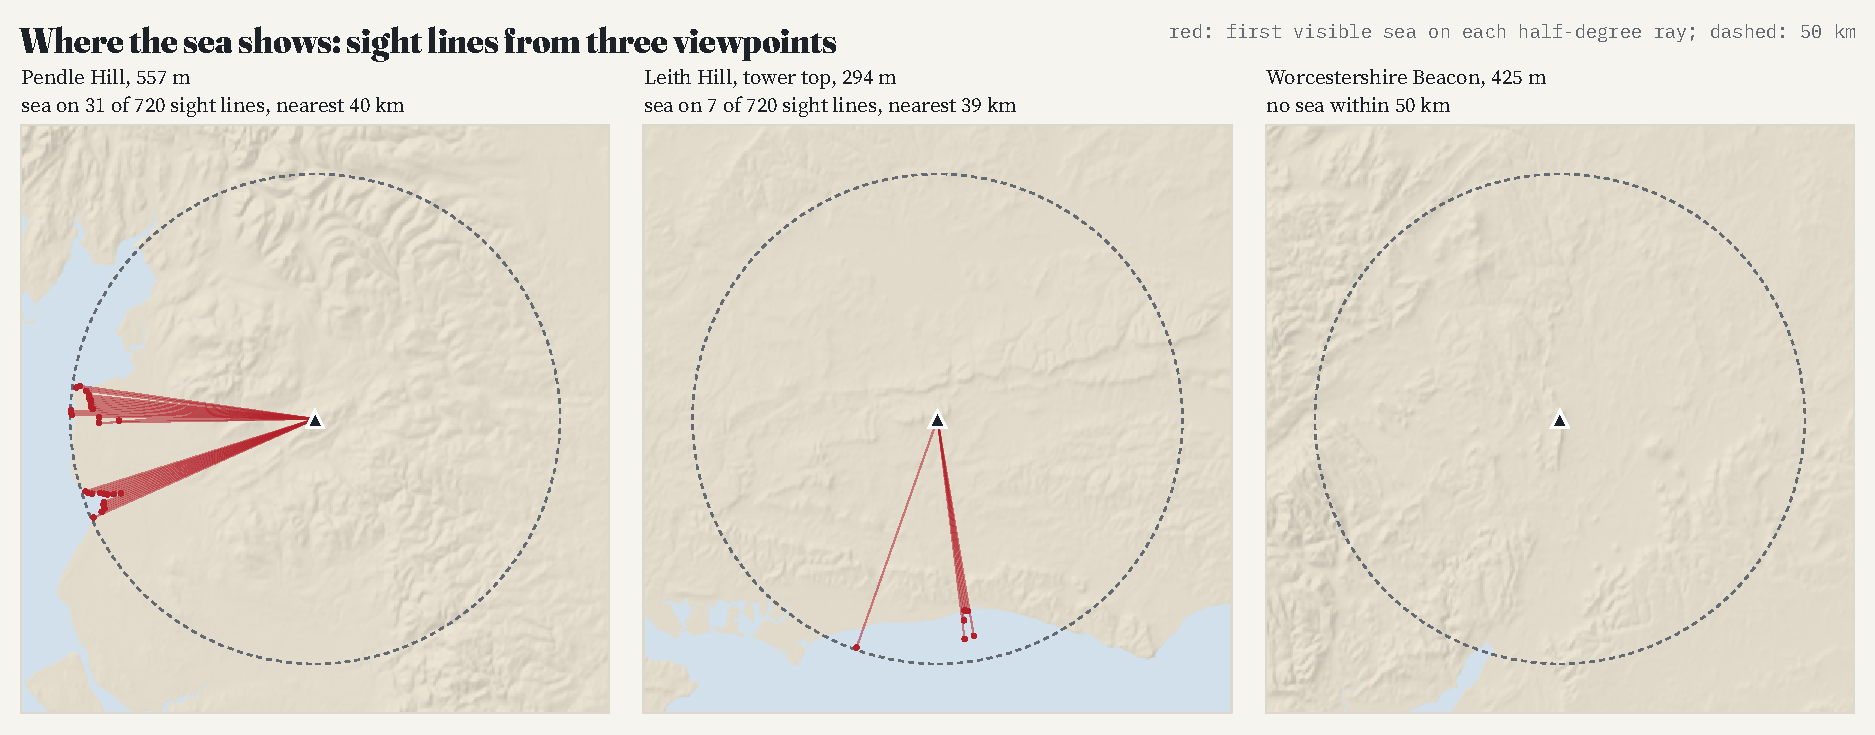
\includegraphics[width=\textwidth]{f_fans.pdf}
\caption{Sight lines from three validation viewpoints at their published heights (Leith Hill: top of the tower), every half degree. Red: the first visible sea on each sight line. Dashed circle: 50~km. Grey: hill shading of the terrain; blue: sea.}\label{fig:fans}
\end{figure}

The plan also called for a check of the farthest point from the coast against a published figure. The Ordnance Survey placed the point in Great Britain farthest from the sea at Church Flatts Farm near Coton in the Elms, Derbyshire (SK~253~144), about 70 miles (113~km) from the sea at mean low water at Fosdyke Wash, near Neston and at Westbury-on-Severn \citep{haran2003}. The square found here lies 114.4~km from the sea, near Akeley (Buckinghamshire), 90~km from the Ordnance Survey point, and the square containing that point is 99~km from the sea here. By the planned rule (more than 10~km apart) this check counts against the coastline used, not the sight lines: OpenStreetMap's coastline follows mean high water and runs far up tidal rivers and estuaries (the same source places the nearest high-tide point to Coton in the Elms on the tidal Trent, about 72~km away), so distances to it are shorter, and the farthest point shifts, compared with a mean-low-water coast. Results that depend on what counts as sea are given with and without narrow channels in Table~\ref{tab:sens}.

\subsection{Sensitivity}
Table~\ref{tab:sens} and Figure~\ref{fig:sens} report the planned checks as changes in the share of land with a sea view, computed on the same squares as the main specification. The headline share ranges from 22.1\% to 27.0\% across them. Limiting the view to 25~km changes it by $-$3.1 points and extending it to 100~km by 0.7: almost all visible sea is close. Refraction matters little ($-$0.7 points without refraction, 0.7 with $k=0.25$). Removing channels narrower than about 1.2~km (a test of whether estuaries and sea lochs count as sea) changes the share by $-$0.8 points: estuaries and narrow sea lochs supply a modest part of the views. Requiring the sea on at least three sight lines changes it by $-$1.3. Doubling the number of rays changes it by 0.2 points on the 5\% sample. On the 500~m grid, 25.8\% of land quarter-points see the sea against 26.4\% of the corresponding square centres, and in 12.1\% of squares the four quarter-points disagree: the 1~km square is a coarse unit at the edges of a view.

The terrain resolution check gives 32.8\% with zoom-10 terrain against 37.0\% with zoom 9 for the same 20,609 squares in the four windows (94.5\% of squares agree; largest window difference 7.3 points). By the planned rule (a difference above 3 points in any window) the headline is therefore resolution-sensitive, and the zoom-10 figures should be read alongside it (Appendix Table~\ref{tab:z10}). The terrain error simulation gives a mean share of 25.2\% (95\% interval 24.6 to 25.8) with 5~m error and 24.7\% (24.0 to 25.3) with 10~m error, against 25.0\% for the same 2,000 squares without error; 12.7\% of squares change their answer in at least one of the 20 realisations with 5~m error, which is the Fisher ``probable viewshed'' margin.

\begin{table}[tbp]\centering\small\caption{Planned sensitivity checks: share of squares (or quarter-points) with a sea view, the difference from the main specification on the same squares (percentage points) and the share of squares with the same answer. Eye height variants are in Table~\ref{tab:nations}.}\label{tab:sens}\begin{tabular}{p{7.2cm}rrrr}\toprule Check & Squares & Sea view (\%) & Difference & Agree (\%)\\\midrule
Main specification & 244,595 & 26.3 & & \\
Maximum distance 25 km & 244,595 & 23.2 & -3.1 & 96.9\\
Maximum distance 100 km & 244,595 & 27.0 & +0.7 & 99.3\\
No refraction (k = 0) & 244,595 & 25.6 & -0.7 & 99.3\\
Strong refraction (k = 0.25) & 244,595 & 27.0 & +0.7 & 99.3\\
Open sea only (channels under about 1 km removed) & 244,595 & 25.4 & -0.8 & 99.2\\
Sea on at least 3 of 360 rays & 244,595 & 25.0 & -1.3 & 98.7\\
720 rays (5\% sample) & 12,229 & 26.5 & +0.2 & 99.8\\
500 m grid (four points per square, 25\% sample) & 61,148 & 25.8 & -0.6 & \\
Terrain at about 88 m (zoom 10), four windows & 20,609 & 32.8 & -4.2 & 94.5\\
Terrain error, sd 5 m (2,000 squares, 20 draws) & 2,000 & 25.2 & +0.2 & \\
Terrain error, sd 10 m (2,000 squares, 20 draws) & 2,000 & 24.7 & -0.3 & \\
\bottomrule\end{tabular}\end{table}

\begin{figure}[tbp]\centering
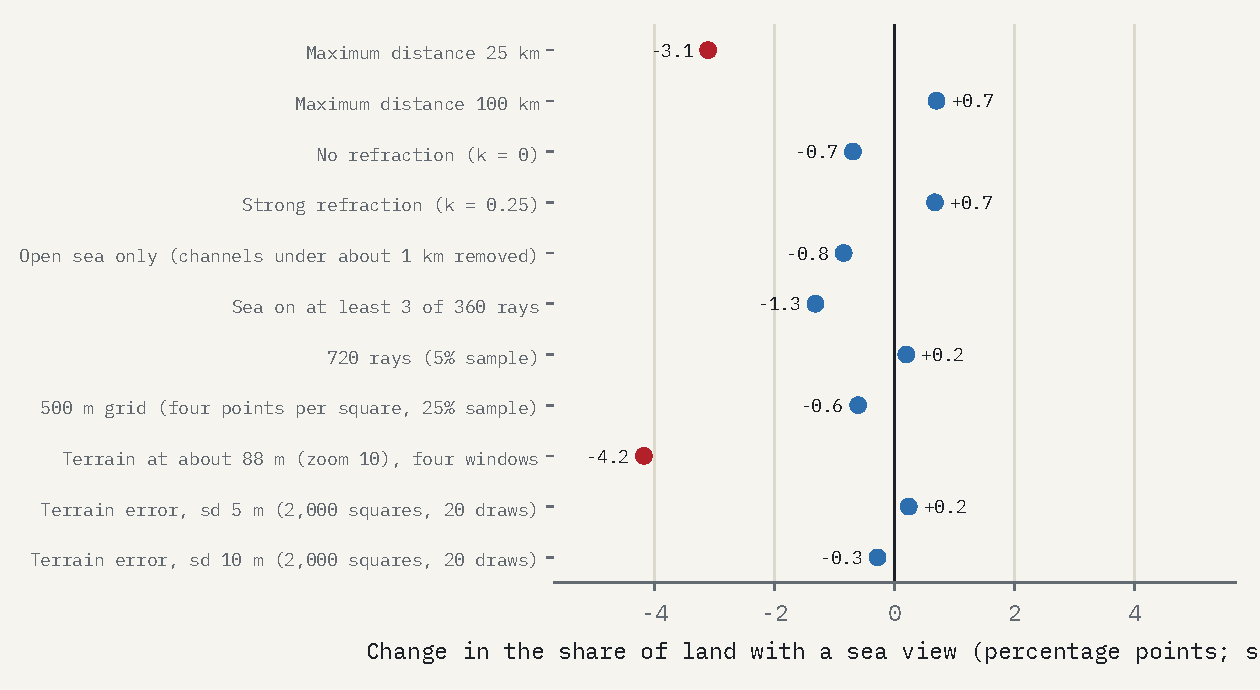
\includegraphics[width=0.85\textwidth]{f_sens.pdf}
\caption{Planned sensitivity checks: change in the share of land with a sea view against the main specification on the same squares (percentage points).}\label{fig:sens}
\end{figure}

\section{Discussion}\label{sec:disc}
The headline, that about a quarter of the UK's land sees the sea from the bare ground (26.3\% with the zoom-9 terrain), is best read as an upper bound on what a person standing outdoors would see on a clear day. Three limitations push in that direction. First, the terrain model has no buildings, hedges or trees as such, and these block most low views in towns and farmland \citep{sander2007}. A sea view from a town's settlement point means that the terrain does not block it, not that a resident can see it from the street. Second, the binary measure counts any visible sea, however small: a sliver of an estuary seen between two hills counts as a view. The share of the horizon and the distance to the nearest visible sea are better measures of how much sea there is to see, and the planned checks show that most of the headline survives requiring more than a glimpse. Third, the air limits what can be seen: haze often hides a sea surface tens of kilometres away, so the 50~km limit is generous on most days, though the 25~km check shows this matters little for the totals.

Other limitations work in both directions. The zoom-9 terrain flattens summits and fills narrow valleys, and it smooths away the low ridges, dunes and embankments that block views from low ground. The resolution check shows the second effect dominating: with terrain at about 88~m the share falls in every test window, by up to 7.3 points (Cornwall) and by $-$4.2 points overall (11\% in relative terms), so the headline is resolution-sensitive. Applying that relative change to the whole country, an exploratory step that assumes the four windows are typical, would give about 23\% rather than 26\%. Lidar terrain at a few metres would probably lower the share again. The coastline is OpenStreetMap's, at mean high water, and includes estuaries and sea lochs; whether a view of the Humber or Loch Long counts as a sea view is a matter of definition, and the open-sea check gives the alternative. The observer stands at the square centre; the 500~m check shows that the answer often differs within a square near the edge of a view, so the per-square result is an indicator for the square, not for every point in it. Tides, which move the water's edge hundreds of metres in places like Morecambe Bay and the Wash, are ignored. Population is attributed through settlement points and Wikidata's patchy population figures; the census weighting within constituencies controls the totals but not where in a constituency people live.

What the measure is good for is comparison and targeting. A per-square indicator with a distance and a horizon share is a better exposure variable for blue-space and hedonic studies than distance to the coast alone, because it distinguishes coastal land that looks out to sea from coastal land that looks inland, and it can be refined with surface models where they exist. The open data and code allow this to be repeated with lidar surface models (which include buildings and trees), with other definitions of the sea or for other countries.

\section{Conclusion}\label{sec:conc}
From 26.3\% of the United Kingdom's land, a person standing on the bare ground could see the sea; from an upstairs window, 29.2\%. Scotland and Wales are sea-view countries; most of England is not. On low ground the view inland fades within about 3~km of the coast, on hills it reaches two to three times as far, and in the English Midlands the nearest square with a sea view can be over 94~km away. All of these figures are upper bounds for bare terrain, and the headline is resolution-sensitive: finer terrain lowered the share in every test window, by up to 7.3 points, so the true bare-ground share is probably below it. ``Sea'' here includes tidal estuaries and sea lochs. The method is simple, exact for the terrain it uses, and ran for the whole country in minutes on two processor cores. Its main limitation, the absence of buildings and trees, is also its clearest direction for further work.

\section*{Data availability}
Data and code: Zenodo DOI https://doi.org/10.5281/zenodo.24106076; also \url{https://github.com/Tristan-Hotham/sea-view}. Interactive map: \url{https://maps.tristanhotham.com/sea-view/}. The written plan that pre-specified the analysis is in NOTES.md in the release. Derived data that depend on the OpenStreetMap coastline are shared under the Open Database Licence.

\section*{AI statement}
I wrote the text, with drafting and editing assistance from Claude (Anthropic), which also helped prepare the analysis code. I reviewed and checked all text and results.

\bibliographystyle{plainnat}
\begin{thebibliography}{99}\small
\bibitem[Amante and Eakins(2009)]{etopo1} Amante, C. and Eakins, B. W. (2009) ETOPO1 1 arc-minute global relief model: procedures, data sources and analysis. NOAA Technical Memorandum NESDIS NGDC-24. National Geophysical Data Center, NOAA. doi:10.7289/V5C8276M.
\bibitem[AWS(2026)]{terraintiles} Registry of Open Data on AWS (2026) Terrain Tiles. \url{https://registry.opendata.aws/terrain-tiles/}
\bibitem[Benedikt(1979)]{benedikt1979} Benedikt, M. L. (1979) To take hold of space: isovists and isovist fields. \textit{Environment and Planning B} 6(1), 47 to 65. doi:10.1068/b060047.
\bibitem[Benson et al.(1998)]{benson1998} Benson, E. D., Hansen, J. L., Schwartz, A. L. and Smersh, G. T. (1998) Pricing residential amenities: the value of a view. \textit{Journal of Real Estate Finance and Economics} 16(1), 55 to 73. doi:10.1023/A:1007785315925.
\bibitem[Bishop(2003)]{bishop2003} Bishop, I. D. (2003) Assessment of visual qualities, impacts, and behaviours, in the landscape, by using measures of visibility. \textit{Environment and Planning B: Planning and Design} 30(5), 677 to 688. doi:10.1068/b12956.
\bibitem[Bourassa et al.(2004)]{bourassa2004} Bourassa, S. C., Hoesli, M. and Sun, J. (2004) What's in a view? \textit{Environment and Planning A} 36(8), 1427 to 1450. doi:10.1068/a36103.
\bibitem[Danielson and Gesch(2011)]{gmted} Danielson, J. J. and Gesch, D. B. (2011) Global multi-resolution terrain elevation data 2010 (GMTED2010). U.S. Geological Survey Open-File Report 2011-1073.
\bibitem[De Floriani and Magillo(2003)]{defloriani2003} De Floriani, L. and Magillo, P. (2003) Algorithms for visibility computation on terrains: a survey. \textit{Environment and Planning B: Planning and Design} 30(5), 709 to 728. doi:10.1068/b12979.
\bibitem[Farr et al.(2007)]{farr2007} Farr, T. G. et al. (2007) The Shuttle Radar Topography Mission. \textit{Reviews of Geophysics} 45(2), RG2004.
\bibitem[Fisher(1991)]{fisher1991} Fisher, P. F. (1991) First experiments in viewshed uncertainty: the accuracy of the viewshed area. \textit{Photogrammetric Engineering and Remote Sensing} 57(10), 1321 to 1327.
\bibitem[Fisher(1992)]{fisher1992} Fisher, P. F. (1992) First experiments in viewshed uncertainty: simulating fuzzy viewsheds. \textit{Photogrammetric Engineering and Remote Sensing} 58(3), 345 to 352.
\bibitem[Fisher(1993)]{fisher1993} Fisher, P. F. (1993) Algorithm and implementation uncertainty in viewshed analysis. \textit{International Journal of Geographical Information Systems} 7(4), 331 to 347. doi:10.1080/02693799308901965.
\bibitem[Fisher(1994)]{fisher1994} Fisher, P. F. (1994) Probable and fuzzy models of the viewshed operation. In Worboys, M. F. (ed.) \textit{Innovations in GIS 1}. London: Taylor and Francis, 161 to 175.
\bibitem[Fisher(1996)]{fisher1996} Fisher, P. F. (1996) Extending the applicability of viewsheds in landscape planning. \textit{Photogrammetric Engineering and Remote Sensing} 62(11), 1297 to 1302.
\bibitem[Franklin and Ray(1994)]{franklin1994} Franklin, W. R. and Ray, C. K. (1994) Higher isn't necessarily better: visibility algorithms and experiments. In Waugh, T. C. and Healey, R. G. (eds) \textit{Advances in GIS Research: Sixth International Symposium on Spatial Data Handling}. London: Taylor and Francis, 751 to 770.
\bibitem[Garrett et al.(2019)]{garrett2019} Garrett, J. K., Clitherow, T. J., White, M. P., Wheeler, B. W. and Fleming, L. E. (2019) Coastal proximity and mental health among urban adults in England: the moderating effect of household income. \textit{Health and Place}, article 102200. doi:10.1016/j.healthplace.2019.102200.
\bibitem[Gascon et al.(2017)]{gascon2017} Gascon, M., Zijlema, W., Vert, C., White, M. P. and Nieuwenhuijsen, M. J. (2017) Outdoor blue spaces, human health and well-being: a systematic review of quantitative studies. \textit{International Journal of Hygiene and Environmental Health} 220(8), 1207 to 1221. doi:10.1016/j.ijheh.2017.08.004.
\bibitem[Gibbons et al.(2014)]{gibbons2014} Gibbons, S., Mourato, S. and Resende, G. M. (2014) The amenity value of English nature: a hedonic price approach. \textit{Environmental and Resource Economics} 57(2), 175 to 196. doi:10.1007/s10640-013-9664-9.
\bibitem[Haklay(2010)]{haklay2010} Haklay, M. (2010) How good is volunteered geographical information? A comparative study of OpenStreetMap and Ordnance Survey datasets. \textit{Environment and Planning B: Planning and Design} 37(4), 682 to 703. doi:10.1068/b35097.
\bibitem[Haran(2003)]{haran2003} Haran, B. (2003) The farm furthest from the sea. BBC News, 23 July 2003. \url{http://news.bbc.co.uk/1/hi/england/derbyshire/3090539.stm}
\bibitem[Hirt et al.(2010)]{hirt2010} Hirt, C., Guillaume, S., Wisbar, A., B\"urki, B. and Sternberg, H. (2010) Monitoring of the refraction coefficient in the lower atmosphere using a controlled setup of simultaneous reciprocal vertical angle measurements. \textit{Journal of Geophysical Research} 115, D21102. doi:10.1029/2010JD014067.
\bibitem[Hotham(2026a)]{hotham2026sunless} Hotham, T. (2026a) Britain's sunless valleys: where hills hide the winter sun. Zenodo. doi:10.5281/zenodo.24055580.
\bibitem[Hotham(2026b)]{hotham2026sunsets} Hotham, T. (2026b) Where the sun sets into the sea: sea sunsets and sunrises at the beaches of Britain and Ireland. Zenodo. doi:10.5281/zenodo.24089892.
\bibitem[Jim and Chen(2009)]{jim2009} Jim, C. Y. and Chen, W. Y. (2009) Value of scenic views: hedonic assessment of private housing in Hong Kong. \textit{Landscape and Urban Planning} 91(4), 226 to 234. doi:10.1016/j.landurbplan.2009.01.009.
\bibitem[Mapzen(2017)]{joerd} Mapzen (2017) Joerd: data sources and attribution for the Terrain Tiles. \url{https://github.com/tilezen/joerd/blob/master/docs/attribution.md}
\bibitem[Nutsford et al.(2016)]{nutsford2016} Nutsford, D., Pearson, A. L., Kingham, S. and Reitsma, F. (2016) Residential exposure to visible blue space (but not green space) associated with lower psychological distress in a capital city. \textit{Health and Place} 39, 70 to 78. doi:10.1016/j.healthplace.2016.03.002.
\bibitem[OpenFreeMap(2026)]{openfreemap} OpenFreeMap (2026) Vector tiles of OpenStreetMap in the OpenMapTiles schema. \url{https://openfreemap.org/}
\bibitem[OpenStreetMap(2026)]{osm} OpenStreetMap contributors (2026) OpenStreetMap. Open Database Licence. \url{https://www.openstreetmap.org/}
\bibitem[Rodriguez et al.(2006)]{rodriguez2006} Rodr\'iguez, E., Morris, C. S. and Belz, J. E. (2006) A global assessment of the SRTM performance. \textit{Photogrammetric Engineering and Remote Sensing} 72(3), 249 to 260. doi:10.14358/PERS.72.3.249.
\bibitem[Sander and Manson(2007)]{sander2007} Sander, H. A. and Manson, S. M. (2007) Heights and locations of artificial structures in viewshed calculation: how close is close enough? \textit{Landscape and Urban Planning} 82(4), 257 to 270. doi:10.1016/j.landurbplan.2007.03.002.
\bibitem[Tabik et al.(2013)]{tabik2013} Tabik, S., Zapata, E. L. and Romero, L. F. (2013) Simultaneous computation of total viewshed on large high resolution grids. \textit{International Journal of Geographical Information Science} 27(4), 804 to 814.
\bibitem[van Kreveld(1996)]{vankreveld1996} van Kreveld, M. (1996) Variations on sweep algorithms: efficient computation of extended viewsheds and class intervals. In \textit{Proceedings of the 7th International Symposium on Spatial Data Handling}, Delft, 15 to 27. Also Utrecht University technical report UU-CS-1996-22.
\bibitem[V\"olker and Kistemann(2011)]{volker2011} V\"olker, S. and Kistemann, T. (2011) The impact of blue space on human health and well-being: salutogenetic health effects of inland surface waters: a review. \textit{International Journal of Hygiene and Environmental Health} 214, 449 to 460.
\bibitem[Vrande\v{c}i\'c and Kr\"otzsch(2014)]{wikidata} Vrande\v{c}i\'c, D. and Kr\"otzsch, M. (2014) Wikidata: a free collaborative knowledgebase. \textit{Communications of the ACM} 57(10), 78 to 85.
\bibitem[Wang et al.(1996)]{wang1996} Wang, J., Robinson, G. J. and White, K. (1996) A fast solution to local viewshed computation using grid-based digital elevation models. \textit{Photogrammetric Engineering and Remote Sensing} 62(10), 1157 to 1164.
\bibitem[Wang et al.(2000)]{wang2000} Wang, J., Robinson, G. J. and White, K. (2000) Generating viewsheds without using sightlines. \textit{Photogrammetric Engineering and Remote Sensing} 66(1), 87 to 90.
\bibitem[Wheatley(1995)]{wheatley1995} Wheatley, D. (1995) Cumulative viewshed analysis: a GIS-based method for investigating intervisibility, and its archaeological application. In Lock, G. and Stan\v{c}i\v{c}, Z. (eds) \textit{Archaeology and Geographical Information Systems: A European Perspective}. London: Taylor and Francis, 171 to 185.
\bibitem[Wheeler et al.(2012)]{wheeler2012} Wheeler, B. W., White, M., Stahl-Timmins, W. and Depledge, M. H. (2012) Does living by the coast improve health and wellbeing? \textit{Health and Place} 18(5), 1198 to 1201. doi:10.1016/j.healthplace.2012.06.015.
\bibitem[White et al.(2010)]{white2010} White, M., Smith, A., Humphryes, K., Pahl, S., Snelling, D. and Depledge, M. (2010) Blue space: the importance of water for preference, affect, and restorativeness ratings of natural and built scenes. \textit{Journal of Environmental Psychology} 30(4), 482 to 493. doi:10.1016/j.jenvp.2010.04.004.
\end{thebibliography}

\appendix
\section{Supplementary tables}
\begin{table}[tbp]\centering\small\caption{Model M1: logistic regression of a square's sea view (1.7~m) on a natural cubic regression spline in log distance to the coast (4 df), log height, local relief and nation (reference England); standard errors clustered by 50~km grid block. N = 244,595 squares, 176 clusters; deviance pseudo-$R^2$ = 0.537.}\label{tab:m1}\begin{tabular}{lrr}\toprule Term & Coefficient & (SE)\\\midrule
Intercept & $-$6.105 & (0.457)\\
Northern Ireland & $-$0.195 & (0.209)\\
Scotland & $-$0.368 & (0.200)\\
Wales & $-$0.377 & (0.229)\\
Spline in log distance, term 0 & $-$3.918 & (0.247)\\
Spline in log distance, term 1 & $-$1.117 & (0.306)\\
Spline in log distance, term 2 & $-$8.735 & (0.335)\\
Spline in log distance, term 3 & $-$17.954 & (3.420)\\
log(1 + height, m) & 0.646 & (0.070)\\
Local relief (m) & 0.008 & (0.001)\\
\bottomrule\end{tabular}\end{table}
\begin{table}[tbp]\centering\small\caption{Counties and council areas (of 79 with at least 200 squares) with the highest and lowest share of land with a sea view at 1.7~m. 18 of 88 areas have no square with a sea view. All areas are in data/counties\_sea.csv.}\label{tab:counties}\begin{tabular}{lrr}\toprule Area & Squares & Sea view (\%)\\\midrule
\multicolumn{3}{l}{\textit{Highest share}}\\
\quad Shetland Islands (Scotland) & 1,491 & 90.7\\
\quad Orkney Islands (Scotland) & 1,035 & 89.6\\
\quad North Ayrshire (Scotland) & 886 & 87.1\\
\quad Na h-Eileanan Siar (Scotland) & 3,086 & 82.9\\
\quad Isle of Wight (England) & 385 & 78.4\\
\quad City of Edinburgh (Scotland) & 261 & 78.2\\
\quad Midlothian (Scotland) & 352 & 77.0\\
\quad East Lothian (Scotland) & 678 & 74.9\\
\multicolumn{3}{l}{\textit{Lowest share}}\\
\quad Bedfordshire (England) & 1,230 & 0.0\\
\quad Cambridgeshire (England) & 3,399 & 0.0\\
\quad Buckinghamshire (England) & 1,881 & 0.0\\
\quad Berkshire (England) & 1,254 & 0.0\\
\quad Derbyshire (England) & 2,628 & 0.0\\
\quad Herefordshire (England) & 2,176 & 0.0\\
\quad Leicestershire (England) & 2,170 & 0.0\\
\quad Hertfordshire (England) & 1,642 & 0.0\\
\bottomrule\end{tabular}\end{table}
\begin{table}[tbp]\centering\footnotesize\setlength{\tabcolsep}{4pt}\caption{Terrain resolution check (S6): squares within 50~km of each window centre, share with a sea view using zoom-9 and zoom-10 terrain (same sea mask), difference (points) and agreement. Coverage: share of the window's pixels with zoom-10 tiles.}\label{tab:z10}\begin{tabular}{lrrrrrr}\toprule Window & Squares & Coverage (\%) & Zoom 9 (\%) & Zoom 10 (\%) & Difference & Agree (\%)\\\midrule
Cumbria and Lancashire coast & 5,688 & 100 & 40.6 & 36.7 & -3.9 & 94.6\\
Cornwall & 3,206 & 89 & 52.5 & 45.2 & -7.3 & 90.2\\
Lothian and Fife & 5,506 & 100 & 51.8 & 47.5 & -4.4 & 94.0\\
Norfolk & 6,209 & 80 & 12.5 & 9.9 & -2.7 & 97.1\\
\bottomrule\end{tabular}\end{table}

\section{Data construction}
\textbf{Terrain mosaic.} The 450 zoom-9 tiles were read from a packed copy of the AWS Terrain Tiles and decoded as $R\times256+G+B/256-32768$ metres. Despiking replaced a cell by its $7\times7$ median where it differed from the median by more than 150~m or stood more than 60~m above (below) the highest (lowest) of its eight neighbours, ignoring the sea floor; four passes. \textbf{Sea mask.} OpenFreeMap vector tiles, water layer, class ocean, rasterised by pixel centre at 256 pixels per tile; tiles were fetched, read and deleted one at a time. \textbf{Squares.} Grid centres were transformed with pyproj (EPSG:27700 and EPSG:29903 to WGS84) and placed in the mosaic; Ireland and the Isle of Man were excluded with Natural Earth polygons. \textbf{Population.} Settlements were assigned to 2010 constituencies by point in polygon (nearest polygon within 3~km for points on the shore). \textbf{Software.} Python with NumPy, SciPy, Numba, pandas, statsmodels, pyproj, rasterio, Shapely and matplotlib; the page uses MapLibre GL JS. Every number in this paper is read from \texttt{data/results.json}.

\end{document}
